\documentclass{article}
\usepackage[utf8]{inputenc}
\usepackage{setspace}
\usepackage{graphicx}
\usepackage{titling}
\usepackage{textcomp}
\usepackage[nottoc]{tocbibind}
\usepackage{tocloft}
\usepackage{natbib}
\usepackage{amsmath}
\usepackage{subcaption}
\renewcommand{\cftsecleader}{\cftdotfill{\cftdotsep}}

\usepackage[margin=1.5in]{geometry}
\addtolength{\topmargin}{-0.5in}
\addtolength{\textheight}{1.0in}

\doublespacing
\newenvironment{bottompar}{\par\vspace*{\fill}}{}

\renewcommand{\contentsname}{\center{Table of Contents}}

\title{Real-time Video Alignment and Fusion Using Feature Detection on FPGA Devices}

\author{Robert Haywood Taglang}

\begin{document}
\pagenumbering{gobble}
\begin{titlingpage}
    \vspace*{\fill}
    \begin{center}
        \textbf{\thetitle}
        
        \hfill \\
        \hfill \\
        
        A Thesis \\
        Submitted to the Faculty \\
        of \\
        Drexel University \\
        by \\
        \theauthor \\
        in partial fulfillment of the \\
        requirements for the degree \\
        of \\
        Master of Science in Computer Engineering \\
        June 2017 \\
    \end{center}
    
    \vspace*{\fill}
    
    \begin{figure*}[!b]
    	\centering
       	
\includegraphics[width=0.35\textwidth]{drexel-vert-blue}
    \end{figure*}
\end{titlingpage}

\begin{center}
	\vspace*{\fill}
	
	\textcopyright\  Copyright 2017
	
	Robert H. Taglang. All Rights Reserved.
	
	\vspace*{\fill}
\end{center}
\clearpage

\pagenumbering{roman}
\setcounter{page}{2}
\begin{center}
    \tableofcontents
    \clearpage
    
    \listoftables
    \clearpage
    
    \listoffigures
\end{center}
\clearpage

\hfill \\
\hfill \\
\hfill \\
\hfill \\

\addcontentsline{toc}{section}{Abstract}

\begin{abstract}
    \singlespacing
    \centering
    \thetitle \\
    \theauthor \\
    Prawat Nagvajara, Ph.D. \\
    
    \hfill \\
    \hfill \\
    \hfill \\
    
    \doublespacing
    Video fusion functions as a way to combine the important or useful parts of two or more sequences of images. The scenario presented is the use of Laplacian fusion to produce a single video composed of the fields of view of two cameras whose areas of focus differ substantially. This is not a useful real-time strategy unless the frames can be aligned. This thesis presents a system for detecting features using an FPGA implementation of SURF (Speeded-Up Robust Features), and aligning video streams by applying a transform generated from the key features. 
\end{abstract}

\clearpage

\pagenumbering{arabic}

\section{Background}

\subsection{Introduction}

The fusion of data from two or more sensors has been well-researched \textit{citations needed}, though these approaches typically discuss the process of fusing images which have been pre-aligned. Pre-computed transforms used to align the frames of two cameras are not robust to variations. Some approaches have made use of additional hardware sensors in order to correct against these variations \cite{chappell_exploiting_2006}. The approach presented in this thesis seeks to perform this correction completely in hardware on a FPGA.

The design choice to use a FPGA rather than a GPU or some other software based approach was made due to the advantages gained from operating with embedded hardware, namely higher portability and lower overall power consumption.

\subsection{Laplacian Fusion}

Laplacian pyramids of images have their origin as a strategy for image encoding \cite{burt_laplacian_1983}. A gaussian blur is applied to the image, and the image is downsampled to half of its original size. This process can be repeated on the resulting image to create a sequence of images representing the original in different scale spaces. This sequence of blurred and downsampled images is known as a Gaussian pyramid. An illustration of a Guassian pyramid for an example image can be seen in Figure \ref{fig_pepper_gaussian_pyramid}.

\begin{figure}[h]
	\centering
	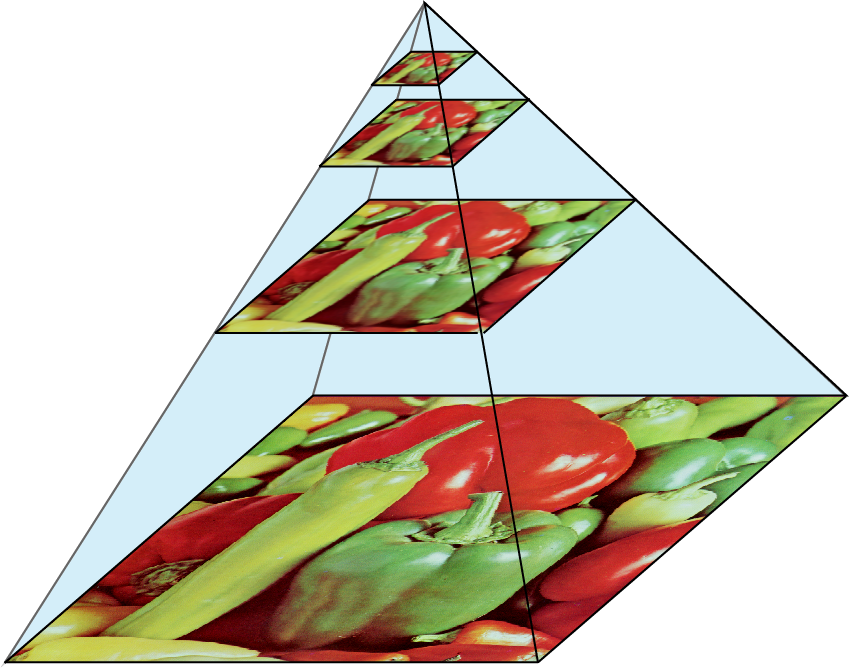
\includegraphics[width=0.6\textwidth]{figures/peppers/gaussian_pyramid}
	\caption{Gaussian pyramid of an example image}
	\label{fig_pepper_gaussian_pyramid}
\end{figure}

The Laplacian pyramid is one which can be used for reconstruction of the original image. At each level above the lowest level of the Gaussian pyramid, the level below is upsampled to match the scale of the current level. The difference between the upsampled image and the current scale level image is known as the Laplacian of the image. The sum of the upsampled lower level and the Laplacian is the original image. At a single level, the Laplacian can be thought of as the error introduced by applying a Gaussian and Box filter. A diagram illustrating a Laplacian pyramid can be seen in Figure \ref{fig_pepper_laplacian_pyramid}

\begin{figure}[h]
	\centering
	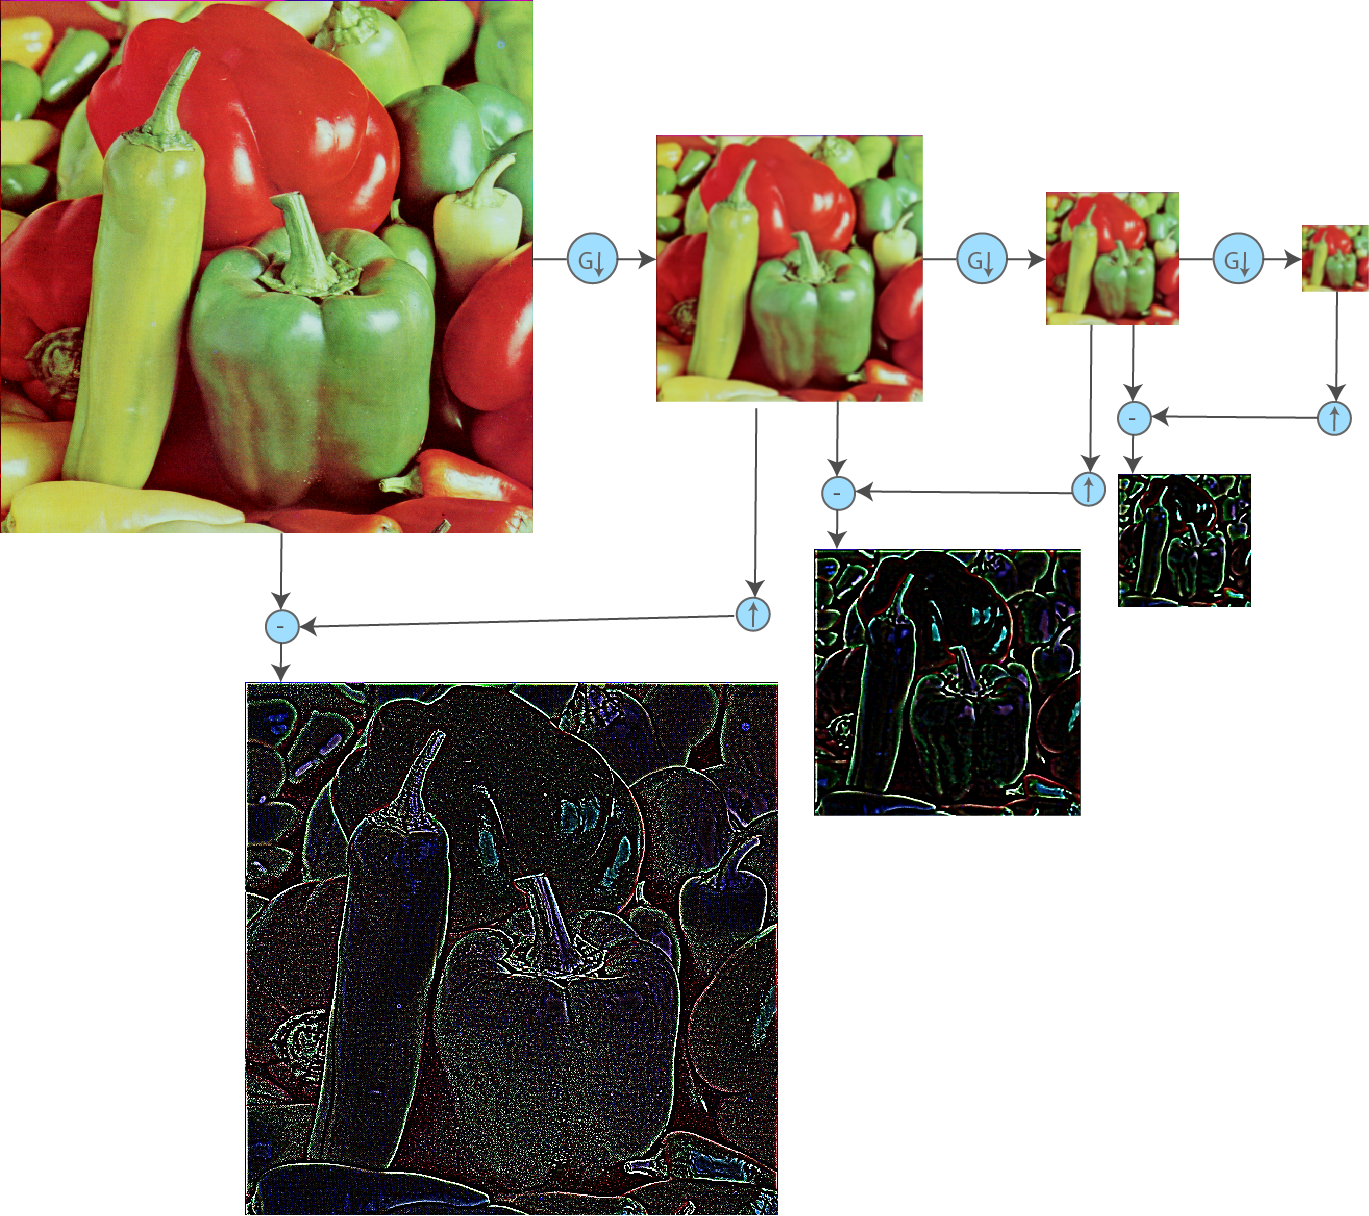
\includegraphics[width=\textwidth]{figures/peppers/laplacian_pyramid}
	\caption{Laplacian pyramid of an example image}
	\label{fig_pepper_laplacian_pyramid}
\end{figure}

The property of the Laplacian that makes it ideal for fusion is its ability to capture the high frequency components in an image through the use of very simple kernel operators that are easily implemented in hardware. The difference between a blurred image and the original will have higher magnitude in the areas where the image was sharpest.

The fusion of two images can be thought of as a function of the two images $X$ and $Y$ of dimension $M \times N$ where $Z = f(X, Y)$ is a single image of dimension $M \times N$. A naive approach to fusion would be to compute the Laplacians and use their magnitudes to select a pixel from either $X$ or $Y$ as shown in Equation \ref{eq_naive_fusion}.

\begin{equation}
Z(i,j)=
\begin{cases}
X(i,j) & |L(X(i,j))| \ge |L(Y(i,j))| \\
Y(i,j) & otherwise
\end{cases}
\label{eq_naive_fusion}
\end{equation}

This approach does not account for variations in colorspace between the two images. Consider the images in Figure \ref{fig_peppers_lr}. The more saturated image will likely have a higher valued Laplacian in some parts simply because it is brighter, therefore having higher magnitudes at individual pixels. This approach also will not facilitate smooth stitching of the images. Contiguous regions of selection from one image will be adjacent to regions from the other with no transition, producing a grainy effect at areas of high frequency. The result of this naive fusion can be seen in Figure \ref{fig_naive_fusion} which exhibits the flaws of this approach.

\begin{figure}[h]
	\centering
	\begin{subfigure}[b]{0.45\textwidth}
		\centering
		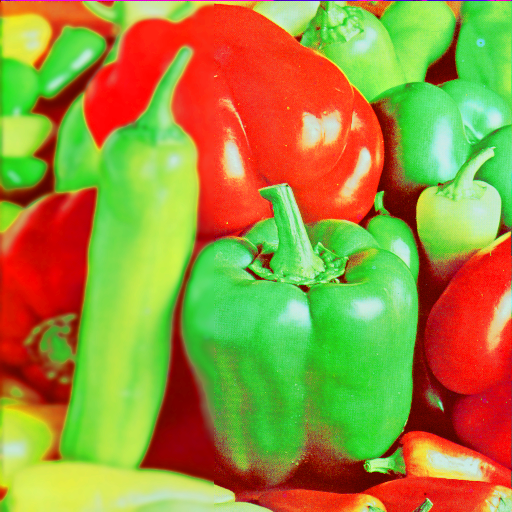
\includegraphics[width=\textwidth]{figures/peppers/peppers_blur_left}
		\caption{Blurred on the left; more saturated}
	\end{subfigure}
	\begin{subfigure}[b]{0.45\textwidth}
		\centering
		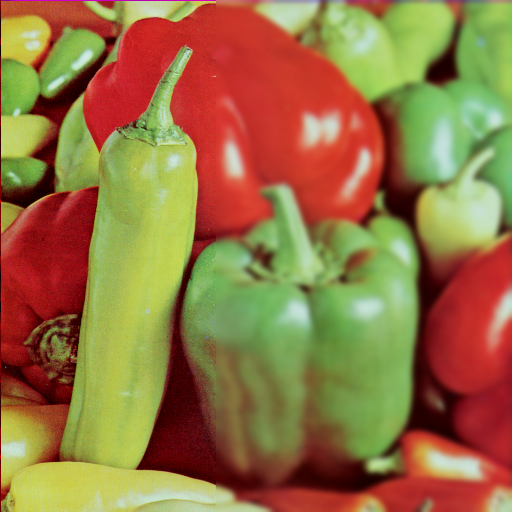
\includegraphics[width=\textwidth]{figures/peppers/peppers_blur_right}
		\caption{Blurred on the right; more neutral}
	\end{subfigure}
	\caption{Two images of the same scene with variations in sharpness and colorspace}
	\label{fig_peppers_lr}
\end{figure}

\begin{figure}[h]
	\centering
	\begin{subfigure}[b]{0.45\textwidth}
		\centering
		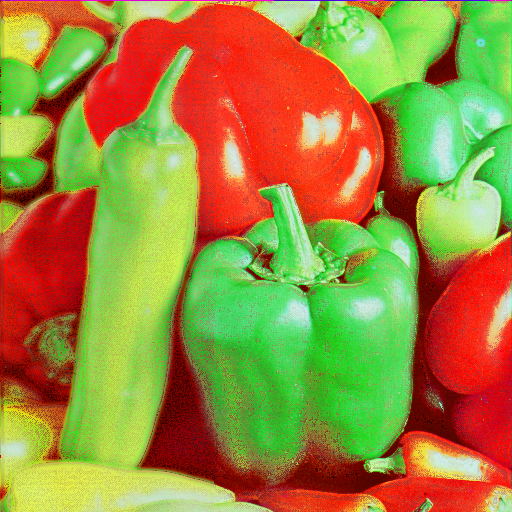
\includegraphics[width=\textwidth]{figures/peppers/peppers_fused_naive}
		\caption{Fusion using the naive approach}
		\label{fig_naive_fusion}
	\end{subfigure}
	\begin{subfigure}[b]{0.45\textwidth}
		\centering
		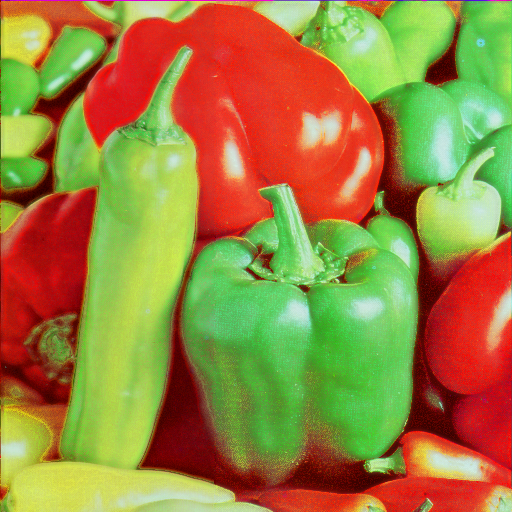
\includegraphics[width=\textwidth]{figures/peppers/peppers_fused}
		\caption{Fusion using weighted sum}
		\label{fig_weighted_fusion}
	\end{subfigure}
	\caption{Fusion of the images in Figure \ref{fig_peppers_lr} using a naive selection and weighted sum approach}
\end{figure}

A more correct approach would involve using the Laplacian as a weight in a weighted sum to combine the pixels of the images, rather than simply selecting them, as shown in Equation \ref{eq_weighted_fusion}.

\begin{equation}
Z(i,j) = \frac{|L(X(i,j))|}{|L(X(i,j))| + |L(Y(i,j))|} \cdot X(i,j) + \frac{|L(Y(i,j))|}{|L(X(i,j))| + |L(Y(i,j))|} \cdot Y(i,j)
\label{eq_weighted_fusion}
\end{equation}

The result of this weighted sum approach can be seen in Figure \ref{fig_weighted_fusion} which exhibits a reduction in graininess from the naive approach.

\subsection{Speeded-up Robust Features (SURF)}

The generation of features for use as marker points in alignment utilizes the SURF algorithm from Bay et al \cite{bay_surf:_2006}. SURF is composed of two parts: a discrete approximation for computing Hessian determinants, and the generation of rotation invariant feature descriptors for detected feature points.

\subsubsection{Computation of Hessian Determinants}

\subsubsection{SURF Implementations for FPGA Devices}

\subsection{Iterative Closest Point Algorithm}

\subsection{Singular Value Decomposition(SVD)}

\subsubsection{SVD Implementations for FPGA Devices}

\section{Implementation}

\subsection{Streaming Kernel Operators}

\subsubsection{Hessian Kernel with Accumulator}

\subsubsection{Box Kernel Approximation of Single Level Laplacian Pyramid}

\subsection{Computation of Transform from Detected Features}

\subsection{Application of Transform to Real-Time Data}

\section{Results}

\pagebreak

\bibliographystyle{plain}
\bibliography{thesis}

\end{document}
